\documentclass{article}
\usepackage[a4paper, left=3cm, right=3cm, top=2.5cm, bottom=2.5cm]{geometry} %Seitenränder
\usepackage[utf8]{inputenc} %Umlaute
\usepackage[T1]{fontenc} %Umlaute 
\usepackage{eurosym} %Eurozeichen
\usepackage[colorlinks=true, linkcolor=black, urlcolor=blue]{hyperref} %Links
\usepackage[ngerman]{babel} % für Deutsche Silbentrennung
\usepackage{listings}
\usepackage[dvipsnames]{xcolor}

% Farben für JavaScript-Code definieren
\definecolor{lightgray}{rgb}{.9,.9,.9}
\definecolor{darkgray}{rgb}{.4,.4,.4}
\definecolor{darkGreen}{rgb}{0.0, 0.5, 0.0}

% JavaScript als neue Sprache definieren
\lstdefinelanguage{JavaScript}{
  keywords={abstract, any, as, boolean, break, case, catch, class, console, 
  const, continue, debugger, declare, default, delete, do, else, enum, export, 
  extends, false, finally, for, from, function, get, if, implements, import, in, 
  infer, instanceof, interface, keyof, let, module, namespace, never, new, null, 
  number, object, package, private, protected, public, readonly, require, return, 
  set, static, string, super, switch, symbol, this, throw, true, try, type, typeof, 
  undefined, unique, unknown, var, void, while, with, yield},
  morecomment=[l]{//},
  morecomment=[s]{/*}{*/},
  morestring=[b]',
  morestring=[b]",
  ndkeywords={class, export, boolean, throw, implements, import, this},
  sensitive=true
}

% Einstellungen für JavaScript-Code
\lstset{
   language=JavaScript,
   backgroundcolor=\color{lightgray},
   extendedchars=true,
   basicstyle=\footnotesize\ttfamily,
   showstringspaces=false,
   showspaces=false,
   numbers=left,
   numberstyle=\footnotesize,
   numbersep=9pt,
   tabsize=2,
   breaklines=true,
   showtabs=false,
   captionpos=b,
   literate=
  {á}{{\'a}}1 {é}{{\'e}}1 {í}{{\'i}}1 {ó}{{\'o}}1 {ú}{{\'u}}1
  {Á}{{\'A}}1 {É}{{\'E}}1 {Í}{{\'I}}1 {Ó}{{\'O}}1 {Ú}{{\'U}}1
  {à}{{\`a}}1 {è}{{\`e}}1 {ì}{{\`i}}1 {ò}{{\`o}}1 {ù}{{\`u}}1
  {À}{{\`A}}1 {È}{{\`E}}1 {Ì}{{\`I}}1 {Ò}{{\`O}}1 {Ù}{{\`U}}1
  {ä}{{\"a}}1 {ë}{{\"e}}1 {ï}{{\"i}}1 {ö}{{\"o}}1 {ü}{{\"u}}1
  {Ä}{{\"A}}1 {Ë}{{\"E}}1 {Ï}{{\"I}}1 {Ö}{{\"O}}1 {Ü}{{\"U}}1
  {â}{{\^a}}1 {ê}{{\^e}}1 {î}{{\^i}}1 {ô}{{\^o}}1 {û}{{\^u}}1
  {Â}{{\^A}}1 {Ê}{{\^E}}1 {Î}{{\^I}}1 {Ô}{{\^O}}1 {Û}{{\^U}}1
  {ã}{{\~a}}1 {ẽ}{{\~e}}1 {ĩ}{{\~i}}1 {õ}{{\~o}}1 {ũ}{{\~u}}1
  {Ã}{{\~A}}1 {Ẽ}{{\~E}}1 {Ĩ}{{\~I}}1 {Õ}{{\~O}}1 {Ũ}{{\~U}}1
  {œ}{{\oe}}1 {Œ}{{\OE}}1 {æ}{{\ae}}1 {Æ}{{\AE}}1 {ß}{{\ss}}1
  {ű}{{\H{u}}}1 {Ű}{{\H{U}}}1 {ő}{{\H{o}}}1 {Ő}{{\H{O}}}1
  {ç}{{\c c}}1 {Ç}{{\c C}}1 {ø}{{\o}}1 {Ø}{{\O}}1 {å}{{\r a}}1 {Å}{{\r A}}1
  {€}{{\euro}}1 {£}{{\pounds}}1 {«}{{\guillemotleft}}1
  {»}{{\guillemotright}}1 {ñ}{{\~n}}1 {Ñ}{{\~N}}1 {¿}{{?`}}1 {¡}{{!`}}1 
}

\lstdefinestyle{JavaScript}{
  language=JavaScript,
  keywordstyle=\color{blue}\bfseries,
  ndkeywordstyle=\color{darkgray}\bfseries,
  identifierstyle=\color{black},
  commentstyle=\color{darkGreen}\ttfamily,
  stringstyle=\color{Bittersweet}\ttfamily,
}

\lstdefinestyle{HTML}{
  language=HTML,
  keywordstyle=\color{blue}\bfseries,
  ndkeywordstyle=\color{darkgray}\bfseries,
  identifierstyle=\color{black},
  commentstyle=\color{darkGreen}\ttfamily,
  stringstyle=\color{Bittersweet}\ttfamily,
}

\lstdefinestyle{CSS}{
  language=css,
  keywordstyle=\color{blue}\bfseries,
  ndkeywordstyle=\color{darkgray}\bfseries,
  identifierstyle=\color{black},
  commentstyle=\color{darkGreen}\ttfamily,
  stringstyle=\color{Bittersweet}\ttfamily,
}
   %Code-Listings für JavaScript (ausgelagert in Listings.tex)

\renewcommand{\familydefault}{\sfdefault} %Schriftart auf serifenlos ändern
\renewcommand{\baselinestretch}{1.15} %Zeilenabstand
\setlength{\parskip}{0.8em} %Absatzabstand
%\setlength{\parindent}{0pt} %kein Einrücken bei neuem Absatz
\title{Devlog - Computer Vision mit openCV.js}
\author{Mattis Thieme}
\date{November 2024}

\begin{document}

\maketitle \newpage

\renewcommand*\contentsname{Inhaltsverzeichnis} %Überschrift des Inhaltsverzeichnisses ändern
\tableofcontents \newpage

\section{Einleitung}

Probleme der Bilderkennung und Bildverarbeitung gewinnen immer mehr an Relevanz. Kein Wunder: Mit der stetigen Verbreitung von mobilen Endgeräten haben immer mehr Systeme Zugriff auf eine (ziemlich hochwertige) Kamera. Die Möglichkeiten, die sich dadurch ergeben, sind vielfältig: über das Scannen von Dokumenten, hin zur Klassifizierung von Tieren und Pflanzen bis hin zum industriellen Einsatz in der Qualitätskontrolle.

Jedoch geht der Trend auch in die Richtung von Onlineservices und Webanwendungen. Programme die früher noch installiert werden mussten, laufen nun direkt im Browser des Clients. Die Gründe sind vielfältig: volle Platformunabhängigkeit, leichtes Einspielen von Updates und keine Installation von zusätzlicher Software. Aber wie sieht es mit Bildverarbeitung und Bilderkennung im Webkontext aus? Die bekannteste Bibliothek für Bildverarbeitung, OpenCV, ist ursprünglich in C++ geschrieben und muss somit auf Serverseite laufen. Aber nicht immer ist die Option sinnvoll oder vorhanden. Nicht immer steht die benötigte Rechenleistung zur Verfügung, auch die Latenz kann letztendlich ein Problem darstellen. Ist es möglich diese Probleme auch im Browser des Clients zu lösen? Die Antwort: Ja! Mit openCV.js.

Ich starte diesen DevBlog um mich genau mit genau dieser Bibliothek auseinanderzusetzen und meine Erfahrungen und Erkenntnisse hier zu teilen. Ich werde genau das gerade erwähnte Problem lösen: Bildverarbeitung direkt im Browser des Clients. Aber was genau möchte ich nun erkennen oder verarbeiten? 

Mein Ziel ist eine Webanwendung, welche Münzen erkennen kann und diese anschließend ihren Wert zuordnet. Warum ausgerechnet Münzen? Zum einen ist es ein recht komplexes Problem, welches gleich viele verschiedene Aspekte der Bildverarbeitung auf Einaml abdeckt, zum anderen ist es eine Problemstellung, welches sich leicht auf einem anderen System reproduzieren lässt. Alles was du brauchst, ist lediglich eine Webkamera und ein paar Münzen. 

Ich habe viele verschieden Ansätze und Ideen, wie ich dieses Problem lösen könnte. Von einfachen Bildoperationen, über die Kreiserkennung bis hin zur Objekterkennung und Musteranalyse. Ob sie alle funktionieren und erfolgreich sind? Keine Ahnung! Jedoch werde ich meine Fortschritte und Erkenntnisse in diesem Blog festhalten und stets meinen Programmcode teilen. Und vielleicht kann ich dir sogar helfen, wenn du vor einem ähnlichen Problem stehen solltest!

Interessiert? Dann lass uns anfangen!

\subsection{Motivation}
Aber warum das ganze? Einst musste ich (wie du vielleicht auch) ein Problem der Bildverarbeitung lösen, welches zwingend im Webkontext stattfinden sollte. Die Anforderungen waren klar: die Bildverarbeitung sollte direkt im Browser des Clients stattfinden, ohne dass der Nutzer eine zusätzliche Software installieren muss. 

Die Bibliothek openCV war natürlich die erste Wahl, jedoch stand ich nun genau vor diesem Problem: wie bekomme ich openCV, eine Bibliothek, die ursprünglich in C++ geschrieben ist, in meiner Webanwendung zum Laufen? Meine Lösung war natürlich openCV.js.

Wenn Probleme im Bereich der Bildverarbeitung gelöst werden sollen, fällt die Wahl häufig auf OpenCV. Und das nicht ohne Grund: OpenCV bietet ein rießiges Spektrum an Funktionen und Algorithmen, von einfachen Bildoperationen hin zu ausgereiften Algorithmen der Gesichtserkennung, Bildsegmentierung und Objekterkennung. Auch Maschinelles Lernen und Deep Learning sind in OpenCV integriert.

Die Wahl der Bibliothek wäre somit schnell getroffen, wenn wir nicht noch ein weiteres Kriterium hätten: die Webanwendung. Da OpenCV jedoch ursprünglich in C++ geschrieben ist, ist das primäre Interface, mit welchem auf die Funktionaltiätenzugegriffen wird, auch in C++ verfasst. Es gibt zwar mit Java und Python auch noch weitere alternative Schnittstellen, jedoch soll unsere Webanwendung, wie bereits oben erwähnt, nicht auf einem Server laufen, sondern direkt im Browser des Clients. Die Lösung: openCV.js.

Als relativ neuer Bestandteil des openCV-Projektes, ist openCV.js eine JavaScript-Portierung der OpenCV-Bibliothek. Sie ermöglicht es, OpenCV-Funktionen direkt im Browser auszuführen, ohne dass der Nutzer eine zusätzliche Software installieren muss. Somit können wir die volle Bandbreite der OpenCV-Funktionen nutzen, ohne auf die Vorteile einer Webanwendung verzichten zu müssen.

Obwohl es sich zunächst als die beste Lösung angehört hat, war die Nutzung von openCV.js jedoch kein Selbstläufer. Wie du wahrscheinlich bereits mit Schrecken festgestellt hast, ist die offizielle Dokumentation nur für die C++ Schnittstelle geschrieben, und Tutorials für openCV.js sind leider rar gesät. Die JavaScript-SChnittstelle von openCV ist nun mal die neuste Änderung des mittlerweise 20 Jahre alten Projektes und somit noch nicht so ausgereift und erprobt wie die anderen Schnittstellen.

Genau aus diesen Gründen habe ich mich für das Schreiben dieses Devlogs entschieden. Ich möchte meine Erfahrungen und Erkenntnisse teilen, um anderen Entwicklern zu helfen, die vor dem gleichen Problem stehen. Ich möchte zeigen, dass es gar nicht so kompliziert ist, openCV.js in einer Webanwendung zu nutzen und wie mächtig die Bibliothek tatsächlich ist. Ja es gibt ein paar Eigenheiten und Macken, aber genau diese werde ich erläutern, damit du nicht die gleichen Fehler machst wie sie ich einst gemacht habe. \newpage

\section{Erstellen der Webseite}

\subsection{openCV.js}
Als aller erstes braucht es natürlich eine aktuelle Version von openCV.js. Diese kann direkt von der offiziellen openCV-Webseite herunterladen:

\href{https://docs.opencv.org/4.10.0/opencv.js}{https://docs.opencv.org/4.10.0/opencv.js}

Es handelt sich hierbei um eine mittels Emscripten kompilierte Version von OpenCV, welche in JavaScript ausgeführt werden kann. Da der Programmcode nur in Bytecode zur Verfügung steht, ist es nicht möglich, den Code direkt zu lesen oder zu verändern. Dies führt zu dem Problem, dass IDE-Funktionalitäten wie Autovervollständigung oder Syntax-Highlighting leider nicht verfügbar sind. 

\subsection{Grundaufbau der Webseite}
Für unsere Webanwendung benötigen wir zunächst eine simple HTML-Struktur mit mindestens zwei Elementen: einem Video-Element für den Kamerastream und einem Canvas-Element, auf welchem wir die Bildverarbeitungsergebnisse anzeigen können. Beide Elemente sollten idealerweise übereinander liegen und die selbe Größe haben.

Nach einigen Tests habe ich mich für folgende Struktur entschieden:
\begin{lstlisting}[style=HTML]
<!DOCTYPE html>
<html lang="de">
<head>
    <meta charset="UTF-8">
    <meta name="viewport" content="width=device-width, initial-scale=1.0">
    <title>Video Player mit Canvas Overlay</title>
    <link rel="stylesheet" href="style.css">
    <script src="lib/opencv_4.10.0.js"></script>
</head>
<body>
<div id="mainContainer">
    <div id="textContainer">
        <h1>CoinFinder</h1>
        <h3>Aktueller Wert: <span id="value">0</span></h3>
    </div>
    <div class="container" id="videoContainer">
        <video id="video" width="720" height="540" autoplay muted loop></video>
        <canvas id="outputCanvas" width="720" height="540"></canvas>
    </div>
</div>
</body>
</html>
\end{lstlisting}

Und die dazugehörige CSS-Datei:

\begin{lstlisting}[style=CSS]
    *{
        box-sizing: border-box;
    }
    
    html, body {
        background-color: #18204d;
        color: #ffffff;
        font-family: Arial, Helvetica, sans-serif;
    }
    
    h3{
        margin: 0 0 0 1em;
    }
    
    #mainContainer{
        position: relative;
        width: 97vw;
        height: 97dvh;
        display: flex;
        flex-direction: column;
    }
    
    #textContainer{
        display: flex;
        align-items: center;
    }
    
    #textContainer > *{
        margin: 0 1em 0 1em;
    }
    
    button{
        background-color: #ffa300;
        color: #18204d;
        border: none;
        padding: 0.5em 1em;
        font-size: 1em;
        cursor: pointer;
    }
    
    #videoContainer{
        position: relative;
        height: 100%;
        width: 100%;
        flex-grow: 1;
        align-items: center;
        justify-content: center;
        display: flex;
    
    }
    
    #video, #outputCanvas {
        height: 100%;
        width: 100%;
        left: 0;
        top: 0;
        position: absolute;
        aspect-ratio: inherit;
        object-fit: contain;
    }
    
    #outputCanvas{
        image-rendering: pixelated;
    }
    
    #mainContainer{
        border: 0.5em solid #ffa300;
    }
    
    #videoContainer{
        border: 0.5em solid blue;
    }
    
\end{lstlisting}

Nun haben wir ein Canvas-Element, welches über dem Video-Element liegt und exakt die selbe Größe hat. Dies ermöglicht es mir, die Bildverarbeitungsergebnisse direkt auf dem dem Canvas zu zeichnen und sie dem Nutzer anzuzeigen. Der Canvas hat zudem die Eigenschaft "image-rendering: pixelated" um auf kleinere Bilder scharf zu zeichnen.

Als nächstes braucht es nun grundlegende Methoden, um auf die Kamera des Nutzers zuzugreifen und den Videostream auf dem Video-Element anzuzeigen.

\subsection{Grundlegende openCV Methoden}
Um auf die Kamera des Nutzers zuzugreifen, kann man unter anderem ein openCV-VideoCapture-Objekt verwenden. Dieses Objekt kann entweder direkt auf ein Video-Element zugreifen oder auf eine Videodatei. Da wir in unserem Fall den Kamerastream verwenden wollen, greifen wir direkt auf das Video-Element zu. Für den Zugriff auf die Webkamera benötigen wir die getUserMedia()-Methode des MediaDevices-Interfaces. Um sicherzustellen, dass openCV vollständig geladen ist, warten wir auf das "load"-Event des Fensters und initialisieren erst dann die Kamera:

\begin{lstlisting}[style=JavaScript]
    window.addEventListener("load", function () {
        video = document.getElementById('video');
        outputCanvas = document.getElementById('outputCanvas');
        videoContainer = document.getElementById('videoContainer');

        // get the camera
        navigator.mediaDevices.getUserMedia({
            video: true,
            audio: false
        }).then(stream => {
            video.srcObject = stream;
            video.onloadedmetadata = () => {
                video.play()

                //print camera stats
                console.log("Camera resolution: " + video.videoWidth + "x" + video.videoHeight);
                console.log("Camera frame rate: " + stream.getVideoTracks()[0].getSettings().frameRate+ " fps");

                //initialize the inputMat-Matrix
                inputMat = new cv.Mat(video.height, video.width, cv.CV_8UC4);
                guiMat = new cv.Mat(video.height, video.width, cv.CV_8UC4);
                videoCapture = new cv.VideoCapture(video);

                //check if everything is loaded
                cameraLoaded = true;
                console.log("Camera loaded");
                CheckIfLoadingFinished();
            };
        }).catch(error => {
            console.error('Error accessing the camera: ', error);
        });
    };
}
\end{lstlisting}

Nachdem die Kamera initialisiert ist, kann die read()-Methode des VideoCapture-Objekts verwendet werden, um den aktuellen Frame des Videostreams in eine openCV-Matrix zu konvertieren. 

Nun brauchen wir jedoch noch eine Methode, um eine openCV-Matrix auf einem Canvas ausgeben zu können. Dafür können wir die cv.imshow()-Methode verwenden, welche eine Matrix auf ein Canvas-Element zeichnet. In unserem Fall verwenden wir das outputCanvas-Element, welches über dem Video-Element liegt. Die Funktion sieht wie folgt aus:

\begin{lstlisting}[style=JavaScript]
function ShowMatrix(src, canvas){
    cv.imshow(canvas, src);
}
\end{lstlisting}

Hinweis zur Speicherfreigabe: openCV.js verwaltet den Speicher nicht automatisch, wie es bei JavaScript üblich ist. Das bedeutet, dass wir selbst dafür verantwortlich sind, den Speicher freizugeben, sobald wir ihn nicht mehr benötigen. Dies betrifft hauptsächlich Objekte vom Typ cv.Mat, welche wir mit der delete()-Methode freigeben können. Tun wir dies nicht, verbraucht der Browser mit jedem neuen Aufruf von new cv.Mat() oder cv.imread() mehr Speicher, bis irgendwann der Browsertab abstürzt. Sollte dein Programm nach einigen Sekunden oder Minuten aufhören zu funktionieren, könnte dies ein Hinweis auf ein Speicherleck sein. Schaue in diesem Fall in die Konsole nach einer entsprechenden Fehlermeldung.

Zu guter Letzt benötigen wir noch einen Hauptloop, welcher die Bilddaten aus dem Video-Element extrahiert, die Kreiserkennung durchführt und das Ergebnis auf dem Canvas-Element anzeigt. Dafür können wir die requestAnimationFrame()-Methode verwenden, welche uns eine optimale Bildwiederholrate garantiert. Ich habe zusätzlich einen Bool "loopActive" hinzugefügt, um den Loop bei Bedarf auch nur einmalig ausführen zu können. Der Loop sieht wie folgt aus:

\begin{lstlisting}[style=JavaScript]
let waitingForAnimationFrame = false;
let angle = 0;
function mainLoop() {
    if(!loadingFinished){
        console.warn("Can't start the loop because something is not loaded yet");
        return;
    }

    waitingForAnimationFrame = false;

    console.log("--- loop started");

    videoCapture.read(inputMat);
    videoCapture.read(guiMat);

    //do something with the matrix
    
    ShowMatrix(guiMat, outputCanvas);

    if(loopActive){
        waitingForAnimationFrame = true;
        requestAnimationFrame(mainLoop);
    }

    console.log("--- loop ended");
}
\end{lstlisting}

Nun sind wir bereit, mit der Kreiserkennung zu beginnen. Im nächsten Abschnitt werden wir uns die Circle Hough Transform genauer ansehen und sie auf unser Beispiel anwenden.
 \newpage

\section{Eingriffe zur Laufzeit}
Halt! Einfach drau los zu programmieren ist nicht immer die beste Idee. Aus Erfahrung weiß ich, dass insbesondere die Arbeit mit OpenCV in viel Trial and Error resultieren kann. 

Bevor ich anfange die ersten Bildverarbeitungsalgorithmen zu implementieren, habe ich daher einige Vorkehrungen getroffen, um den Entwicklungsprozess zu beschleunigen und zu vereinfachen. In diesem Abschnitt möchte ich näher auf diese Vorkehrungen eingehen, und zudem verdeutlichen warum es bei der Arbeit mit OpenCV so wichtig ist, einfache Testing-Möglichkeiten zu haben.

\subsection{Die Bedeutung von einfachem Testing}
Meine nächste Aufgabe, die Implementierung der Kreiserkennung, erfordert eine Menge an Feintuning und Anpassungen. Jeder Parameter muss sorgfältig gewählt werden, um ein optimales Ergebnis zu erzielen. Zudem kann ich vorhinein nicht ermittelt werden, welche Parameter die besten sind. Es ist also ein iterativer Prozess, bei dem ich die Parameter anpasse, das Ergebnis betrachte und dann erneut die Parameter anpasse.

Nun stelle man sich vor, man müsste für jede kleine Änderung die Webseite neu laden, die Kamera neu ausrichten und die Münzen neu platzieren. Dies ist der Grund, weshalb ich Eingriffe zur Laufzeit implementieren möchte. Diese Eingriffe sollen es mir ermöglichen, die Parameter der Kreiserkennung und weiterer openCV Funktionen direkt zur Laufzeit zu verändern, ohne die Webseite neu laden zu müssen, und somit schnell die besten Parameter zu finden.

\subsection{Variablen-Slider}
Meine Idee ist es, einen HTML-Slider erstellen zu können, mit dem ich schnell und einfach den Wert einer beliebigen JS-Variable verändern kann. Diese Slider sollen sowohl den aktuellen Wert der Variable anzeigen als auch bei Interaktion des Benutzers ihre zugewiesene Variable verändern. Der Wert des HTMl-Elementes soll somit direkt mit der Variable synchronisiert werden.

Für die Slider habe ich die Bibliothek \href{https://refreshless.com/nouislider/}{noUISlider} verwendet.  Über die data-Attribute von den HTML-Elementen kann unkompliziert der Wertebereich und die Schrittweite des Sliders festgelegt werden.

Nun müsste aber standardmäßg ein Event-Listener für jeden Slider erstellt werden, der bei Veränderung den Wert einer Variable ändert. Da ich jedoch nicht für jede Variable einen eigenen Event-Listener erstellen möchte, habe ich mich für einen anderen Ansatz entschieden. Stattdessen soll man direkt im HTML-Element des Sliders angeben können, welche Variable durch diesen Slider verändert werden soll.

Hierfür benötigen wir zunächst ein eigenes data-Attribute , in welchem der Name der zu verändernen Varaible angegeben wird. Zum Zweiten benötigen wir eine Funktion, die alle Slider-Elemente durchgeht und für jedes Element mithilde des data-Attributs den Event-Listener für die angegebene Variable erstellt. Hierfür braucht es eine Möglichkeit den String-Namen der Variable in eine Referenz auf die Variable umzuwandeln. Dies kann mithilfe der \texttt{eval()}-Funktion erreicht werden.

Die Event-Listener Funktion sieht dann wie folgt aus:

\begin{lstlisting}[style=JavaScript]
function InitSliders(){
    // Alle Slider-Container selektieren
    const sliderContainers = document.querySelectorAll('.sliderContainer');

    sliderContainers.forEach(container => {
        const sliderElement = container.querySelector('.slider');
        const valueElement = container.querySelector('.sliderValue');

        const min = parseFloat(container.dataset.min);
        const max = parseFloat(container.dataset.max);
        const step = parseFloat(container.dataset.step);
        const var1 = container.dataset.var1;
        const var2 = container.dataset.var2;
        const isRange = container.dataset.range === "true"; // Überprüft, ob Bereichsmodus aktiv ist
        //console.log("Data for slider: min: " + min + " max: " + max + " step: " + step + " var1: " + var1 + " var2: " + var2 + " isRange: " + isRange);

        // Startwerte auslesen
        let startValues = [];
        if (isRange) {
            // Bereichsmodus: Startwerte aus den <span>-Elementen lesen
            const spanValues = valueElement.querySelectorAll('span');
            startValues = Array.from(spanValues).map(span => parseFloat(span.textContent));
            if (startValues.length !== 2) {
                // Fallback: Standardwerte in der Mitte des Bereichs
                startValues = [min + (max - min) / 3, max - (max - min) / 3];
            }
        } else {
            // Einzelregler: Einzelwert auslesen
            startValues = [parseFloat(valueElement.textContent) || (min + max) / 2];
        }

        // Slider erstellen
        noUiSlider.create(sliderElement, {
            start: startValues,
            range: {
                'min': min,
                'max': max
            },
            step: step,
            connect: isRange ? true : [true, false] // Verbindet die Regler bei Range-Modus
        });

        SetSliderValueFromCookie(container.id);

        // Update-Event
        sliderElement.noUiSlider.on('update', (values, handle) => {
            if (isRange) {
                // Bereichsmodus: Werte in <span>-Elementen aktualisieren
                if(step >= 1){
                    valueElement.textContent = values.map(value => Math.round(value)).join(' - ');
                }else{
                    valueElement.textContent = values.map(value => value).join(' - ');
                }

                //TODO: Beide Variablen aktualisieren
                if(var1 !== undefined && var2 !== undefined){
                    UpdateVariable(var1, values, 0);
                    UpdateVariable(var2, values, 1);
                }else{
                    console.log("var1 or var2 is undefined. Slider will not change any variables");
                }


            } else {
                // Einzelregler: Textinhalt aktualisieren
                if(step >= 1){
                    valueElement.textContent = Math.round(values[handle]);
                }else{
                    valueElement.textContent = values[handle];
                }

                if(var1 !== undefined){
                    // Variable aktualisieren
                    UpdateVariable(var1, values, handle);
                }else{
                    console.log("var1 is undefined. Slider will not change any variables");
                }

            }

            // Cookie setzen
            SetSliderCookie(container.id, values);
        });
    });

    console.log("Sliders initialized");
}
\end{lstlisting}

Die Funktion UpdateVariable() wandelt schließlich den String-Namen der Variable in eine Referenz um und ändert den Wert der Variable. Hierfür wird die eval()-Funktion verwendet, die den String als JavaScript-Code interpretiert.

\begin{lstlisting}[style=JavaScript]
function UpdateVariable(varName, values, handle){
    //check if variable exists
    if (eval('typeof ' + varName) === 'undefined') {
        console.warn('Variable '+varName+' does not exist');
        return;
    }

    //update variable
    if(eval('typeof ' + varName) === 'number'){
        eval(varName + ' = ' + parseFloat(values[handle]));
    }else if(eval('typeof ' + varName) === 'string'){
        eval(varName + ' = ' + values[handle]);
    }
}
\end{lstlisting}

Wie du vielleicht gesehen hast, gibt es auch noch die Funktionen SetSliderValueFromCookie() und SetSliderCookie(). Diese Funktionen dienen dazu, die Werte der Slider in Cookies zu speichern und beim Laden der Webseite wiederherzustellen. So behalten die Slider ihre eingestellten Werte auch nach einem Neuladen der Webseite.

\subsection{Cookies}

Cookies sind kleine Textdateien, die auf dem Computer des Benutzers gespeichert werden. Wie du sicherlich bereits weißt, dienen sie unter anderem dem Zweck, Informationen Session-übergreifend zu speichern. In meinem Fall möchte ich die Werte der Slider speichern, um sie beim Neuladen der Webseite wiederherzustellen.

Jedoch ist das Speichern von Werten in Cookies nicht ganz trivial: Pro Cookie kann nur ein einziger String mit einer maximalen Länge von 4096 Bytes gespeichert werden. Da die Werte der Slider jedoch Arrays von Zahlen sind, müssen diese erst in einen String umgewandelt werden. Hierfür habe ich mich für die JSON.stringify()-Funktion entschieden, die ein JavaScript-Objekt in einen JSON-String umwandelt. Die Funktion zum schreiben des Cookies sieht dann wie folgt aus:

\begin{lstlisting}[style=JavaScript]
function SetSliderCookie(sliderId, value) {
    // Holen des bestehenden Cookie-Werts
    let sliderValues = GetSliderCookie();

    // Setze den Wert des Sliders im Cookie
    sliderValues[sliderId] = value;

    // Setze den Cookie mit den neuen Werten
    const expires = new Date();
    expires.setDate(expires.getDate() + 7); // Cookie läuft in 7 Tagen ab
    document.cookie = `sliderValues=${JSON.stringify(sliderValues)}; expires=${expires.toUTCString()}; path=/;`;
}
\end{lstlisting}

Zunächst erstelle ich ein Objekt "sliderValues" aus dem Cookie, falls es bereits existiert. Anschließend füge ich den neuen Wert des Sliders hinzu und speichere das Objekt als JSON-String im Cookie. Hierfür muss zudem ein Ablaufdatum für den Cookie festgelegt werden, in meinem Fall läuft der Cookie nach 7 Tagen ab. Der Cookie sieht dann wie folgt aus:

\begin{lstlisting}[style=JavaScript]
{"slider1":["5100.00"],"slider2":["3900.00"],"slider3":["7.00"],"slider4":["3.00"],"sliderValue3":["230.00"],"sliderValue4":["129.00"]}
\end{lstlisting}

Um die Daten aus dem Cookie wiederherzustellen, muss in der Funktion GetSliderCookie() der Cookie ausgelesen und in ein JavaScript-Objekt umgewandelt werden. Eine saubere Lösung, welche selbst beim Vorhandensein von weiteren Cookies funktioniert, könnte wie folgt aussehen:

\begin{lstlisting}[style=JavaScript]
function GetSliderCookie(){
    const value = `; ${document.cookie}`;
    const parts = value.split(`; sliderValues=`);
    if (parts.length === 2) {
        const cookieValue = parts.pop().split(';').shift();
        return JSON.parse(cookieValue);  // Parsen des JSON-Strings
    }
    return {};  // Falls der Cookie nicht existiert, ein leeres Objekt zurückgeben
}
\end{lstlisting}

Lass mich diese Funktion kurz erklären: Zunächst wird der Cookie-Wert aus dem document.cookie-String extrahiert. Die \enquote{cookie} Eigenschaft des Objekts \enquote{document} enthält alle Cookies, die auf der aktuellen Seite gesetzt wurden. Dem String wird ein Semikolon und ein Leerzeichen vorangestellt, um sicherzustellen, dass der Cookie-Wert korrekt extrahiert wird, selbst wenn noch andere Cookies vorhanden sind. Nun wird über value.split('; sliderValues=') der String zweigeteilt. Der erste Teil, welcher alles vor dem Cookie-Wert enthält, wird per pop() verworfen. Der zweite Teil, welcher den Cookie-Wert inklusive möglicher weiterer Cookies enthält, muss noch weiter verarbeitet werden. Hierfür wird der String per split(';') wieder in ein Array geteilt und mit shift() das erste Element, welches den Cookie-Wert enthält, extrahiert. Nun erst können wir sicher sein, dass mögliche weitere Cookies vor und nach unserem Cookie-Wert entfernt wurden. Der Slider-Cookie-Wert wird schließlich per JSON.parse() in ein JavaScript-Objekt umgewandelt und zurückgegeben.

Zu guter Letzt braucht es noch eine Funktion, welche beim Start der Webseite die Werte der Slider aus dem Cookie wiederherstellt. Diese Funktion sieht wie folgt aus:

\begin{lstlisting}[style=JavaScript]
function SetSliderValueFromCookie(containerID){
    const sliderValues = GetSliderCookie();
    const sliderContainer = document.getElementById(containerID);

    if (!sliderContainer) {
        console.error('Slider container not found');
        return;
    }

    const slider = sliderContainer.querySelector('.slider');
    const sliderValueElement = sliderContainer.querySelector('.sliderValue');

    if (!slider || !sliderValueElement) {
        console.error('Slider or value element not found');
        return;
    }

    const savedValue = sliderValues[containerID];

    if (savedValue !== undefined) {
        // Den Slider auf den gespeicherten Wert setzen
        slider.noUiSlider.set(savedValue);

        // Anzeige des aktuellen Werts aktualisieren
        sliderValueElement.textContent = Array.isArray(savedValue) ? savedValue.join(' - ') : savedValue;
    }else{
        console.log("No saved value for " + containerID + " found in cookie");
    }
}
\end{lstlisting}

Nun habe ich endlich eine solide Möglichkeit geschaffen, schnell und unkompliziert Variablen zur Laufzeit zu verändern und diese Änderungen sogar über einen Neustart der Webseite hinweg zu speichern. Dies wird mir hoffentlich eine Menge Zeit und Nerven sparen, wenn ich nun im nächsten Blogeintrag mit der Implementierung der Kreiserkennung beginne. \newpage

\section{Kreiserkennung}

\subsection{Funktionsweise der HoughCircles-Methode}
Das Implementieren der Kreiserkennung in openCV.js war tatsächlich ziemlich einfach. Alles was es grundsätzlich dafür braucht ist diese Methode:

\begin{lstlisting}[style=JavaScript]
cv.HoughCircles(image, circles, method, dp, minDist, param1, param2, minRadius, maxRadius);
\end{lstlisting}

Gehen wir erstmal die einzelnen Parameter durch:
\begin{itemize}[label={}]
    \item \textbf{image} - Dies ist das Bild, in dem die Kreise gefunden werden sollen. Es muss eine openCV-Matrix sein und sollte als Graustufenbild vorliegen.
    \item \textbf{circles} - In diese Matrix werden die gefundenen Kreise gespeichert. Ja - die Methode schreibt die Kreise direkt in eine openCV-Matrix. In OpenCV können Matrizen nicht nur für die Speicherung von Bildern verwendet werden, sondern auch für die Speicherung von Vektoren. In diesem Fall wird in der Matrix \enquote{circles} in jeder Zeile ein Kreis gespeichert. Ein Kreis ist dabei ein Vektor der Form \([x, y, r]\), wobei \((x, y)\) die Koordinaten des Mittelpunkts des Kreises und \(r\) der Radius des Kreises sind.
    
    Weiter unten zeige ich eine Möglichkeit, wie die einzelnen Kreise in dieser Matrix in Objekte umgewandelt werden können. Dies macht die weitere Verarbeitung der Kreise deutlich einfacher.
    \item \textbf{method} - Dies ist eine Konstante, die angibt, welche Methode zur Kreiserkennung verwendet werden soll. In openCV.js gibt es aktuell nur eine Methode, die verwendet werden kann, nämlich \texttt{cv.HOUGH\_GRADIENT}.
    \item \textbf{dp} - Hier wird es leider etwas komplizierter. Der Parameter \texttt{dp} ist ein inverser Skalierungsfaktor, der die Genauigkeit der Kreiserkennung beeinflusst. Ein Wert von 1 bedeutet, dass die Auflösung des Eingabebildes verwendet wird. Ein Wert von 2 bedeutet, dass das Eingabebild halb so groß wie das Originalbild ist. Je kleiner der Wert, desto genauer ist die Kreiserkennung, aber auch desto langsamer. 
    \item \textbf{minDist} - Dieser Parameter gibt den minimalen Abstand zwischen den Mittelpunkten der gefundenen Kreise an. Dies ist sehr nützlich um die Anzahl an falschen Positiven zu reduzieren. 
    \item \textbf{param1} - Dieser Parameter ist spezifisch für die Methode \texttt{cv.HOUGH\_GRADIENT}. Es handelt sich hier um den oberen Schwellwert für die Kantenerkennung, welche intern durchgeführt wird. Der untere Schwellwert ist stets die Hälfte dieses Wertes.
    \item \textbf{param2} - Dieser Parameter ist ebenfalls spezifisch für die Methode \texttt{cv.HOUGH\_GRADIENT}. Er ist der Schwellwert für die Kreiserkennung. Je kleiner der Wert, desto empfindlicher ist die Kreiserkennung, d.h. ein Kreis muss weniger stark ausgeprägt sein, um trotzdem als solcher erkannt zu werden. Dies bedeutet jedoch auch, dass das mit kleinerem Wert das Risiko für falsche Kreise steigt.
\end{itemize}

Der Einfachheit halber habe ich eine eigene Methode nur für das Finden von Kreisen geschrieben, die die Methode \texttt{cv.HoughCircles} verwendet. Diese Methode gibt dann ein Array von Kreis-Objekten zurück, die ich dann weiterverarbeiten kann. Die Methode sieht so aus:

\begin{lstlisting}[style=JavaScript]
function FindCircles(inputMat, guiMat){

    //Eingabe-Matrix in Graustufen umwandeln
    cv.cvtColor(inputMat, grayMat, cv.COLOR_RGBA2GRAY);

    //reset circlesMat
    circlesMat.delete();
    circlesMat = new cv.Mat();

    //Hough-Transformation
    cv.HoughCircles(grayMat, circlesMat, cv.HOUGH_GRADIENT, dp, minRadius, param1, param2, minRadius, maxRadius);

    //create circle objects
    let foundCircles = [];
    for (let i = 0; i < circlesMat.cols; ++i) {
        let x = circlesMat.data32F[i * 3];
        let y = circlesMat.data32F[i * 3 + 1];
        let radius = circlesMat.data32F[i * 3 + 2];

        foundCircles.push(new Circle(x, y, radius));
    }

    //draw circles
    for(let i = 0; i < foundCircles.length; i++){
        DrawCircle(foundCircles[i], guiMat, [255,255,255,255]);
    }

    return foundCircles;
}
\end{lstlisting}

Auch für das Anzeigen der Kreise habe ich eine ausgelagerte Methode geschrieben. Dies wäre eigentlich nicht nötig gewesen, da für das Zeichnen von Kreisen nur eine einziger Methodenaufruf benötigt wird. Ich habe die Methode dennoch geschrieben, um die Lesbarkeit des Codes zu erhöhen. Die Methode sieht so aus:

\begin{lstlisting}[style=JavaScript]
function DrawCircle(circle, guiMat, color){
    //return if parameter is not set
    if(circle === undefined){
        console.error("Circle is undefined");
        return;
    }

    //draw circle
    cv.circle(guiMat, new cv.Point(circle.x, circle.y), circle.radius, color, 2);
}
\end{lstlisting}

Bei den Parametern \texttt{dp}, \texttt{param1} und \texttt{param2} stellte sich mir nun die Frage, welche Werte ich hier verwenden soll. Eine pauschale Antwort darauf gibt es nicht, da die optimalen Werte stark vom Bild, vom Verwendungszweck und in meinem Beispiel auch von der Kamera abhängen.

Meine nächste Aufgabe war es nun, für meinen Anwendungsfall die optimalen Werte für diese Parameter zu finden. Hierfür habe ich den Mainloop so angepasst, dass in einer Schleife die Kreiserkennung auf dem aktuellen Kamera-Frame durchgeführt wird. Die gefundenen Kreise werden dann auf eine separate "GUI-Matrix" gezeichnet, die dann auf dem Bildschirm angezeigt wird. Durch das Verändern der Parameter per Slider konnte ich so direkt die Auswirkungen auf die Kreiserkennung sehen.

Letztendlich habe ich bei diesen Werten sehr gute Ergebnisse erzielt:
\begin{itemize}
    \item \texttt{dp} = 2
    \item \texttt{minDist} = 18
    \item \texttt{param1} = 230
    \item \texttt{param2} = 129
    \item \texttt{minRadius} = 18
    \item \texttt{maxRadius} = 67
\end{itemize}

Dies bedeutet nicht, dass diese Werte auch für andere Anwendungsfälle optimal sind. Je nach Lichtverhältnissen, Kamerawinkel und Bildqualität können diese Werte stark variieren. Es ist also sehr wichtig, die Parameter für die Kreiserkennung an jeden Anwendungsfall individuell anzupassen.

\subsection{Buffering der Kreise} \newpage

\section{Histogramme}

\subsection{Überlegungen}
Jetzt wo ich die Kreiserkennung implementiert habe, ist es mir möglich Münzen im Bild zu erkennen. Der nächste Schritt wäre es nun, die Münzen zu klassifizieren und zu unterscheiden. Doch wie klassifiziert man in openCV Bilder? Meine Idee war es, die Bilder als Histogramme zu speichern und zu vergleichen. Ein Histogramm ist eine graphische Darstellung der Häufigkeitsverteilung von Werten. In meinem Fall würde ich die Farbwerte der Münzen in einem Histogramm speichern und diese dann vergleichen.

\subsection{Die Vorlagen}
Damit ich die Münzen anhand ihrer Bildinformastionen klassifizieren kann, benötige ich zuerst Vorlagen, mit denen ich die Münzen vergleichen kann. Ich habe also Bilder von den Münzen gemacht und diese als Vorlagen gespeichert. Diese Vorlagenbilder sind die Referenzbilder, anhand derer ich die Münzen im Kamerabild auf Ähnlichkeit überprüfen möchte.

Hier hat sich vorallem die spiegelnde Oberfläche der Münzen als Problem herausgestellt. Ich musste viel mit dem Lichteinfallswinkel und der Beleuchtung spielen, um von jeder Münze ein gutes Bild zu bekommen. Auch der Abnutzungsgrad hat das Erstellen der Vorlagen erschwert. So musste ich vorallem bei den 50-20-10 Cent Münzen und bei den 5-2-1 Cent Münzen darauf achten, dass die Münzen stets eine ähnliche Optik ausweisen. Andernfalls könnte es passieren, dass die Spiegelung oder die Abnutzung als Unterschied interpretiert wird und nicht mehr die Ziffern auf den Münzen.

Meine Vorlagen sehen wie folgt aus:

\begin{figure}[ht]
    \centering
    \begin{subfigure}{0.23\textwidth}
        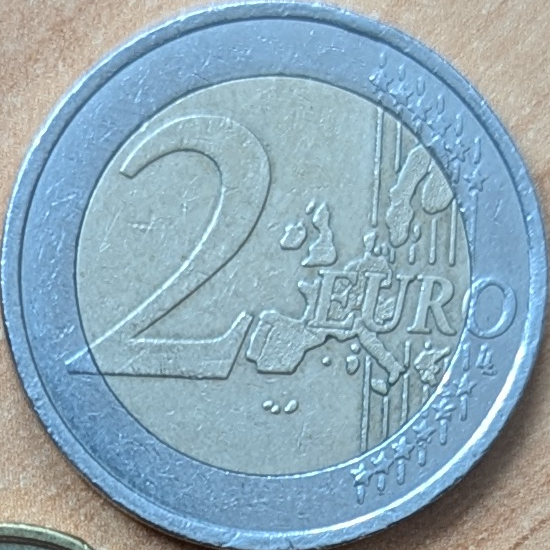
\includegraphics[width=\linewidth]{../CoinFinder/templates_2/Euro2.png}
    \end{subfigure}
    \begin{subfigure}{0.23\textwidth}
        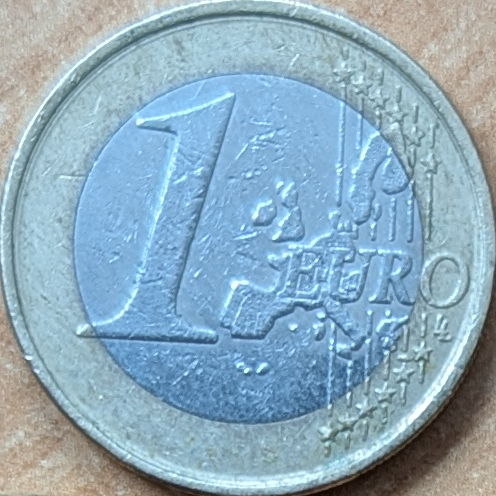
\includegraphics[width=\linewidth]{../CoinFinder/templates_2/Euro1.png}
    \end{subfigure}
    \begin{subfigure}{0.23\textwidth}
        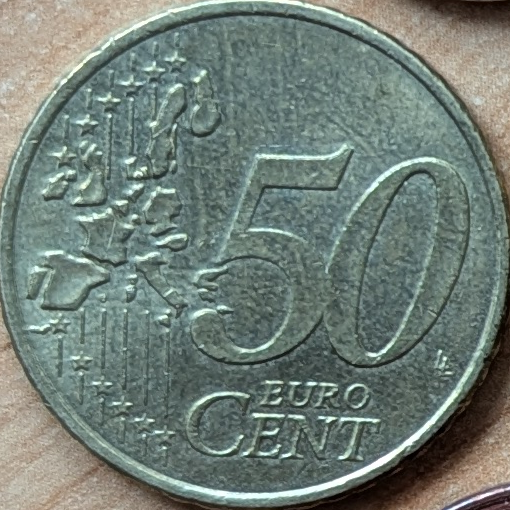
\includegraphics[width=\linewidth]{../CoinFinder/templates_2/Cent50.png}
    \end{subfigure}
    \begin{subfigure}{0.23\textwidth}
        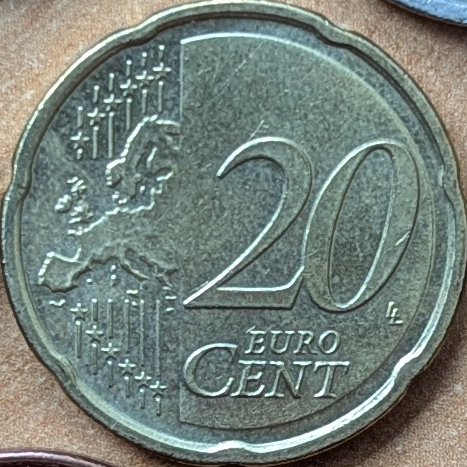
\includegraphics[width=\linewidth]{../CoinFinder/templates_2/Cent20.png}
    \end{subfigure}

    \begin{subfigure}{0.23\textwidth}
        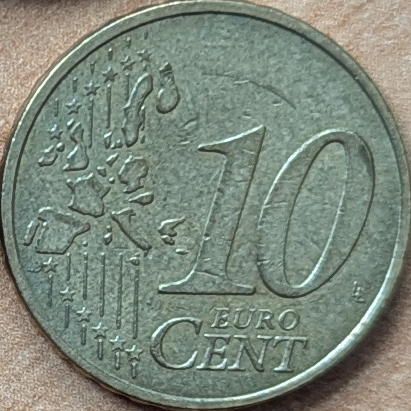
\includegraphics[width=\linewidth]{../CoinFinder/templates_2/Cent10.png}
    \end{subfigure}
    \begin{subfigure}{0.23\textwidth}
        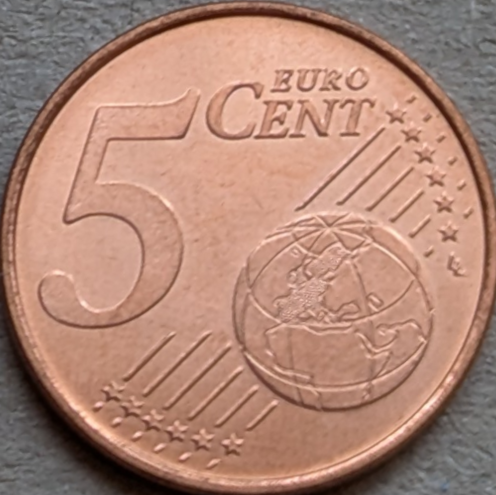
\includegraphics[width=\linewidth]{../CoinFinder/templates_2/Cent5.png}
    \end{subfigure}
    \begin{subfigure}{0.23\textwidth}
        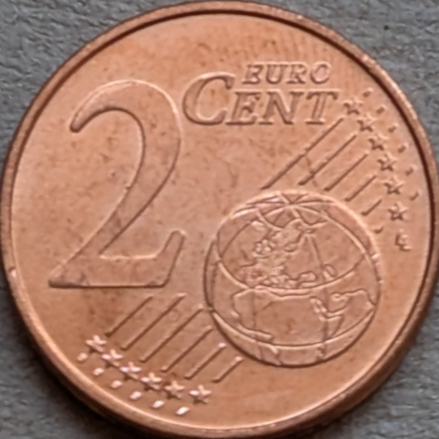
\includegraphics[width=\linewidth]{../CoinFinder/templates_2/Cent2.png}
    \end{subfigure}
    \begin{subfigure}{0.23\textwidth}
        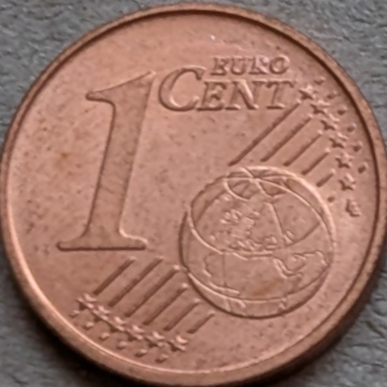
\includegraphics[width=\linewidth]{../CoinFinder/templates_2/Cent1.png}
    \end{subfigure}
\end{figure}

\subsection{Erstellung der Histogramme}

\subsection{Vergleich der Histogramme}

\subsection{Erste Ergebnisse} \newpage

\section{Template Matching}

\subsection{Überlegungen}
Jetzt wo ich die Kreiserkennung implementiert habe, ist es mir möglich Münzen im Bild zu erkennen. Der nächste Schritt wäre es nun, die Münzen zu klassifizieren und zu unterscheiden. Doch wie klassifiziert man in openCV Bilder? Eine Möglichkeit ist das Template Matching. Dabei wird ein Template, also eine Vorlage, über ein Bild geschoben und die Ähnlichkeit an jedem Punkt beziehungsweise Pixel berechnet. Das Ergebnis ist eine Heatmap, die die Übereinstimmung an jedem Punkt im Bild anzeigt.

\subsection{Die Vorlagen}
Damit ich die Münzen anhand ihrer Bildinformastionen klassifizieren kann, benötige ich zuerst Vorlagen, mit denen ich die Münzen vergleichen kann. Ich habe also Bilder von den Münzen gemacht und diese als Vorlagen gespeichert. Diese Vorlagenbilder sind die Referenzbilder, anhand derer ich die Münzen im Kamerabild auf Ähnlichkeit überprüfen möchte.

Hier hat sich vorallem die spiegelnde Oberfläche der Münzen als Problem herausgestellt. Ich musste viel mit dem Lichteinfallswinkel und der Beleuchtung spielen, um von jeder Münze ein gutes Bild zu bekommen. Auch der Abnutzungsgrad hat das Erstellen der Vorlagen erschwert. So musste ich vorallem bei den 50-20-10 Cent Münzen und bei den 5-2-1 Cent Münzen darauf achten, dass die Münzen stets eine ähnliche Optik ausweisen. Andernfalls könnte es passieren, dass die Spiegelung oder die Abnutzung als Unterschied interpretiert wird und nicht mehr die Ziffern auf den Münzen.

Meine Vorlagen sehen wie folgt aus:

\begin{figure}[ht]
    \centering
    \begin{subfigure}{0.23\textwidth}
        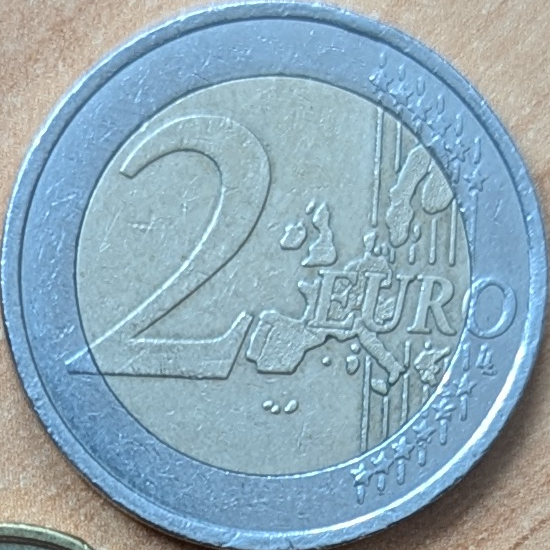
\includegraphics[width=\linewidth]{../CoinFinder/templates_2/Euro2.png}
    \end{subfigure}
    \begin{subfigure}{0.23\textwidth}
        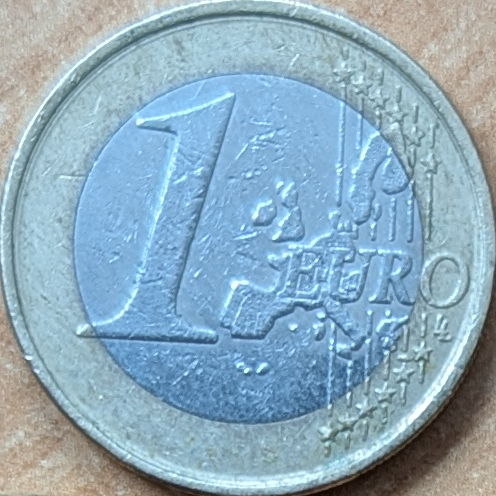
\includegraphics[width=\linewidth]{../CoinFinder/templates_2/Euro1.png}
    \end{subfigure}
    \begin{subfigure}{0.23\textwidth}
        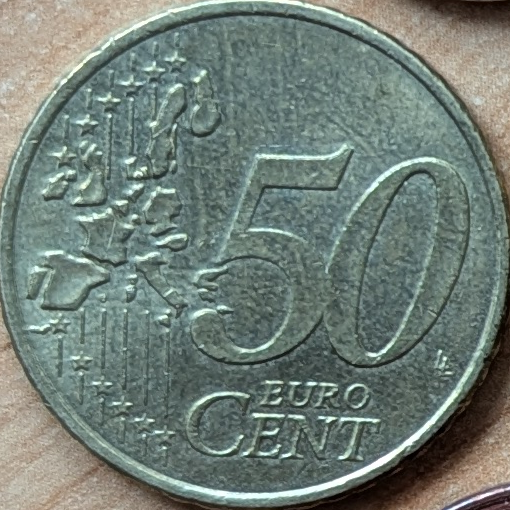
\includegraphics[width=\linewidth]{../CoinFinder/templates_2/Cent50.png}
    \end{subfigure}
    \begin{subfigure}{0.23\textwidth}
        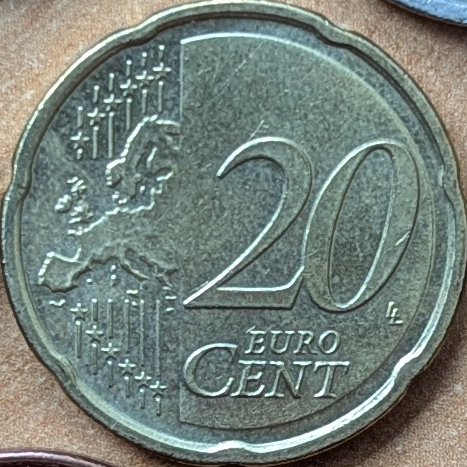
\includegraphics[width=\linewidth]{../CoinFinder/templates_2/Cent20.png}
    \end{subfigure}

    \begin{subfigure}{0.23\textwidth}
        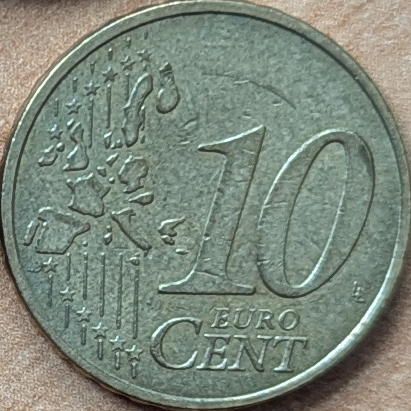
\includegraphics[width=\linewidth]{../CoinFinder/templates_2/Cent10.png}
    \end{subfigure}
    \begin{subfigure}{0.23\textwidth}
        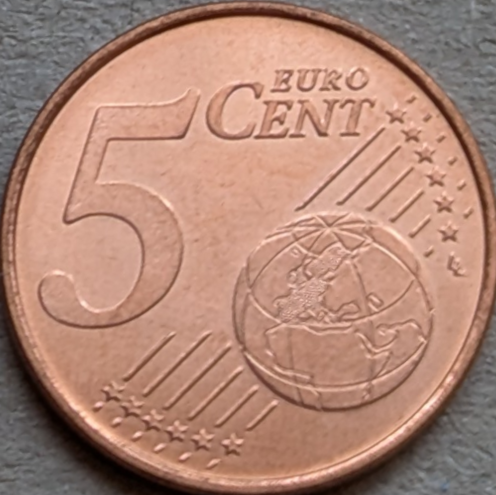
\includegraphics[width=\linewidth]{../CoinFinder/templates_2/Cent5.png}
    \end{subfigure}
    \begin{subfigure}{0.23\textwidth}
        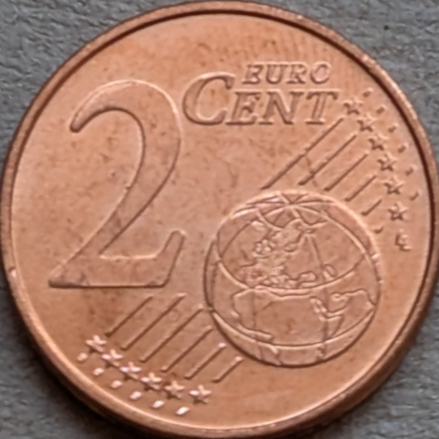
\includegraphics[width=\linewidth]{../CoinFinder/templates_2/Cent2.png}
    \end{subfigure}
    \begin{subfigure}{0.23\textwidth}
        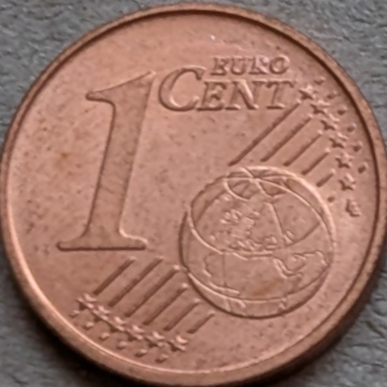
\includegraphics[width=\linewidth]{../CoinFinder/templates_2/Cent1.png}
    \end{subfigure}
\end{figure}

Bevor ich nun mit dem Vergleich der Vorlagen beginne, brauche ich zunächst eine Möglichkeit um sowohl die Vorlagen als auch die daraus resultierenden Ergebnisse zu speichern. Dafür habe ich ein global verfügbares Objekt \textit{COINS} erstellt, welches die Münzen als Schlüssel enthält und als Wert ein Objekt mit den Eigenschaften \textit{diameter} und \textit{value} hat. Weitere Eigenschaften können dann zur Laufzeit den einzelnen Münzen hinzugefügt werden.

\begin{lstlisting}[style=JavaScript]
let COINS = {
    Euro2 : {
        diameter: 25.75,
        value: 2
    },
    Euro1 : {
        diameter: 23.25,
        value: 1
    },
    Cent50 : {
        diameter: 24.25,
        value: 0.5
    },
    Cent20 : {
        diameter: 22.25,
        value: 0.2
    },
    Cent10 : {
        diameter: 19.75,
        value: 0.1
    },
    Cent5 : {
        diameter: 21.25,
        value: 0.05
    },
    Cent2 : {
        diameter: 18.75,
        value: 0.02
    },
    Cent1 : {
        diameter: 16.25,
        value: 0.01
    }
}    
\end{lstlisting}

Diese Datenstruktur kann ich nun verwenden, um die Vorlagen zu speichern und ihnen eine Münze zuzuordnen. In der folgenden Methode iteriere ich über jede Münze und lese das Vorlagenbild ein:

\begin{lstlisting}[style=JavaScript]
const templatesLoaded = new Event('templatesLoaded');
let path = "../Templates/"

function InitTemplates() {
    let coinLength = Object.keys(COINS).length;
    let loadedCoins = 0;
    Object.entries(COINS).forEach(([key, value]) => {
        //is in the template folder a picture with the same name as the key?
        let img = new Image();

        img.onload = () => {
            //save image as matrix in the coin object
            COINS[key].template = cv.imread(img);

            loadedCoins++;
            if(loadedCoins === coinLength){
                document.dispatchEvent(templatesLoaded);
            }
        }

        img.onerror = () => {
            console.log("error: " + key);
        }

        img.src = path + key + ".png";

    });
}
\end{lstlisting}

Das Event \textit{templatesLoaded} wird ausgelöst, sobald alle Vorlagen geladen wurden. Somit kann ich sicherstellen, dass Programmschritt welche die Vorlagen benötigen erst ausgeführt werden, wenn die Vorlagen auch wirklich geladen wurden.
\subsection{Funktionsweise}
Template Matching funktioniert in openCV.js mit der folgenden Funktion:
\begin{lstlisting}[style=JavaScript]
cv.matchTemplate(image, templ, result, method, mask);
\end{lstlisting}

Lasst uns die Parameter genauer betrachten:
\begin{itemize}
    \item \textbf{image} - Das Bild, in dem das Template gesucht werden soll. Es muss als openCV-Matrix vorliegen.
    \item \textbf{templ} - Das Template, das gesucht werden soll. Es muss auch als openCV-Matrix vorliegen.
    \item \textbf{result} - Die Heatmap, in der die Übereinstimmung an jedem Punkt im Bild gespeichert wird. Auch diese muss als openCV-Matrix vorliegen.
    \item \textbf{method} - Die Methode, die zur Berechnung der Übereinstimmung verwendet werden soll. Aktuell gibt es folgende Methoden in openCV.js:
    \subitem \textbf{cv.TM\_SQDIFF} - Summe der quadrierten Differenzen (kleinere Werte bedeuten bessere Übereinstimmung)
    \subitem \textbf{cv.TM\_SQDIFF\_NORMED} - Normalisierte Summe der quadrierten Differenzen (kleinere Werte bedeuten bessere Übereinstimmung)
    \subitem \textbf{cv.TM\_CCORR} - Kreuzkorrelation (größere Werte bedeuten bessere Übereinstimmung)
    \subitem \textbf{cv.TM\_CCORR\_NORMED} - Normalisierte Kreuzkorrelation (größere Werte bedeuten bessere Übereinstimmung)
    \subitem \textbf{cv.TM\_CCOEFF} - Kreuzkorrelationskoeffizient (größere Werte bedeuten bessere Übereinstimmung)
    \subitem \textbf{cv.TM\_CCOEFF\_NORMED} - Normalisierter Kreuzkorrelationskoeffizient (größere Werte bedeuten bessere Übereinstimmung)
    \item \textbf{mask} - (optional) Eine Maske, die angibt, welche Bereiche des Bildes berücksichtigt werden sollen. In meinem Fall benutze ich keine Maske, da ich bereits vor Aufruf der Funktion unwerwünschte Bereiche des Bildes ausschneide.
\end{itemize}

Meine Funktion für das Template Matching sieht nun so aus:
\begin{lstlisting}[style=JavaScript]
function MatchTemplates(src, circle){
    //create result string
    let resultsString = [];
    Object.entries(COINS).forEach(([key, value]) => {
        let resultMat = new cv.Mat();

        //resize template to the size of src
        let templateResized = new cv.Mat();
        cv.resize(COINS[key].template, templateResized, COINS[key].template.size(), 0, 0, cv.INTER_AREA);

        cv.matchTemplate(src, templateResized, resultMat, cv.TM_SQDIFF_NORMED);

        //get highest value
        let minMax = cv.minMaxLoc(resultMat);
        let min = minMax.minVal;

        resultsString.push(new Result(key, min));

        templateResized.delete();
    });

    //sort results from highest to lowest
    resultsString.sort((a, b) => a.value - b.value);

    //console.dir(resultsString);

    //save bestmatch in circle
    circle.bestMatch = COINS[resultsString[0].name];
    circle.matchValue = resultsString[0].value;

    //set matchValue to 2 decimal places
    circle.matchValue = Math.round(circle.matchValue * 100) / 100;

    src.delete();
}
\end{lstlisting}

Innerhalb des main-loops wird diese Funktion nun für jeden gefundenen Kreis ausfgerufen. Der Parameter "src" ist dabei eine ausgeschnittene Region des Bildes, in der sich der Kreis befindet. Der Parameter "circle" ist das Circle-Objekt, in dem die Informationen zum Kreis gespeichert sind. Die Funktion iteriert anschließend über alle Vorlagen und berechnet die Übereinstimmung für jede Vorlage. Hierbei muss beachtet werden, dass Vorlage und das zu prüfende Bild vorher auf die selbe Größe gebracht werden müssen. Die Ergebnisse werden in einem Array gespeichert und anschließend sortiert. Das beste Ergebnis wird dann im Circle-Objekt gespeichert.

\subsection{Exkurs: Mehrere Matrizen in einem Canvas anzeigen}
Bei wachsender Komplexität der Webanwendung ob ich mir immer wieder gewünscht eine Möglichkeit zu haben, mehrere Matrizen in einem Canvas anzuzeigen. Dies ist standardmäßig in openCV.js nicht vorgesehen, da die Funktion \textit{cv.imshow()} immer nur eine Matrix anzeigen kann. Also habe ich mir eine eigene Funktion geschrieben, die mehrere Matrizen in einem Canvas anzeigen kann. Diese Funktion sieht so aus:

\begin{lstlisting}[style=JavaScript]
function ShowMatrices(src, canvas) {
    if (src.length === 0) {
        console.error("No src to show");
        return;
    }

    if (src.length === 1) {
        console.warn("Only one matrix to show. Using ShowMatrix instead");
        ShowMatrix(src[0], canvas);
        return;
    }

    let numberOfMatrices = src.length;

    // Berechnung der Gittergröße
    let gridCols = Math.ceil(Math.sqrt(numberOfMatrices));
    let gridRows = Math.ceil(numberOfMatrices / gridCols);

    // Maximalbreite und -höhe der Matrizen basierend auf der Größe des Canvas
    let cellWidth = canvas.width / gridCols;
    let cellHeight = canvas.height / gridRows;

    // Canvas leeren
    let ctx = canvas.getContext('2d');
    ctx.clearRect(0, 0, canvas.width, canvas.height);

    // Jede Matrix im Gitter zeichnen
    src.forEach((mat, index) => {
        // Spalte und Zeile bestimmen
        let col = index % gridCols;
        let row = Math.floor(index / gridCols);

        // Zielbereich für diese Matrix
        let x = col * cellWidth;
        let y = row * cellHeight;
        let targetSize = new cv.Size(cellWidth, cellHeight);

        // Matrix auf passende Größe skalieren
        let resizedMat = new cv.Mat();
        cv.resize(mat, resizedMat, targetSize, 0, 0, cv.INTER_AREA);

        // Matrix in RGBA umwandeln wenn es sich um eine Graustufenmatrix handelt
        if (resizedMat.channels() === 1) {
            let rgbaMat = new cv.Mat();
            cv.cvtColor(resizedMat, rgbaMat, cv.COLOR_GRAY2RGBA);
            resizedMat.delete();
            resizedMat = rgbaMat;
        }

        // Erstelle ein temporäres Canvas für diese Matrix
        let tempCanvas = document.createElement('canvas');
        let tempCtx = tempCanvas.getContext('2d');
        tempCanvas.width = resizedMat.cols;
        tempCanvas.height = resizedMat.rows;

        // In ein ImageData konvertieren und in das temporäre Canvas zeichnen
        let imageData = new ImageData(new Uint8ClampedArray(resizedMat.data), resizedMat.cols, resizedMat.rows);
        tempCtx.putImageData(imageData, 0, 0);

        // Zeichne das temporäre Canvas auf das Haupt-Canvas
        ctx.drawImage(tempCanvas, 0, 0, resizedMat.cols, resizedMat.rows, x, y, cellWidth, cellHeight);

        // Bereinige die temporären Matrizen
        resizedMat.delete();
    });
}
\end{lstlisting}

Um mehrere Bilder in einen Canvas zu zeichnen, musste ich die Größe der Bilder anpassen, damit sie in ein Grid passen. Dafür habe ich die Funktion \textit{cv.resize()} verwendet. Anschließend müssen die Matrizen zuerst in ein temporäres Canvas gezeichnet werden, bevor sie in das Haupt-Canvas gezeichnet werden können. Die Funktion \textit{drawImage()} von Canvas kann nur Bilder zeichnen, keine Matrizen. Daher musste ich die Matrizen in ein ImageData-Objekt umwandeln, bevor ich sie in das Canvas zeichnen konnte.
\subsection{Erste Ergebnisse}
Es hat sich gezeigt, dass der Vergleich der Vorlagen prinzipiell funktionieren kann. Jedoch ist die Genauigkeit  noch nicht zufriedenstellend. Münzen können zwar grob in die richtige Kategorie eingeordnet werden (sprich 1-2-5 Cent Münzen und 10-20-50 Cent Münzen), jedoch ist die Unterscheidung innerhalb dieser Kategorien nicht funktional. So werden aktuell nur maximal die Hälfte der Münzen korrekt zugeordnet.

Es scheint, als wären die Informationen der Ziffern auf den Münzen nicht ausreichend, um eine genaue Klassifizierung zu ermöglichen. Die Farbe einer Münze hat im Gegensatz dazu einen relativ großen Einfluss auf das Ergebnis. So werden Münzen meist der korrekten Farbkategorie zugeordnet, jedoch nicht derm korrekten Wert. Dies ist ein Hinweis darauf, dass die Farbinformationen der Münzen stärker gewichtet werden als die Forminformationen. Da sich Münzen innerhalb einer Kategorie (z.B. 1-2-5 Cent Münzen) jedoch nur in der Größe und ihrer Ziffer optisch unterscheiden, ist es schwierig eine weitere Methode der Klassifizierung zu finden. Ein Prüfen der Größe würde in meinem Anwendungsfall nicht funktionieren, da sowohl der Abstand zur Kamera als auch die Position der Münzen im Bild variabel sind. 

Eine Möglichkeit die Genauigkeit zu erhöhen wäre es, den störenden Faktor der Farbinformationen zu eliminieren, und stattdessen nur Vorlagen zu verwenden, welche nur die notwendigen Informationen enthalten. Dies könnte z.B. durch das Erstellen von Kantenbildern der Münzen erreicht werden. Solche Bilder wie sie vom Canny-Algorithmus erstellt werden, enthalten nur die Kanten des Ausgangsbildes und keine Farbinformationen, da sie rein als Schwarz-Weiß-Bilder vorliegen. Diese Kantenbilder könnten dann an Stelle der aktuellen Farbbilder als Vorlagen verwendet werden.

Jedoch gibt es noch ein weiteres Problem: die Rotation. Bereits eine kleine Drehung des Ausgangsbildes verursacht große Unterschiede in der Übereinstimmung. Das Template Matching in openCV berechnet standardmäßig nur die Übereinstimmung für das Template in der gleichen Rotation wie das Bild. Dies ist ein Problem, da die Münzen im Kamerabild in unterschiedlichen Rotationen vorkommen können. Eine Möglichkeit dieses Problem zu lösen wäre es, das Template in verschiedenen Rotationen zu speichern und für jede Rotation die Übereinstimmung zu berechnen. Dies würde jedoch die Anzahl der Vorlagen vervielfachen und einen unverhältnismäßig hohen Aufwand bedeuten. Eine andere Möglichkeit wäre es, das Ausgangsbild mehrfach zu rotieren und für jede Rotation die Übereinstimmung zu den Vorlagen berechnen. So wäre bei ausreichend kleingranularer Rotation sichergestellt, dass jede Münze mindestens einmal eine ähnliche Ausrichtung wie das zutreffende Template hat. Dies würde jedoch die Rechenzeit signifikant erhöhen, da bedeutend mehr Berechnungen pro Münze durchgeführt werden müssten. Zudem braucht es dafür eine Möglichkeit, alle Zwischenergebnisse der Rotationen zu speichern, um anschließend das beste Ergebnis zu wählen. \newpage

\section{Anpassungen}

\subsection{Kantenerkennung}

\subsubsection{Funktionsweise der Canny-Methode}
\subsubsection{Die korrekten Parameter finden}

\subsection{Matrizen rotieren und transformieren}

\subsection{Neues Problem: Mat-Types}

\subsection{Asynchronität und Ladebalken} \newpage

\section{Ergebnisse}

\subsection{Neue MatchTemplate-Funktion}
Meine finale MatchTemplate-Funktion sieht nun so aus:

\begin{lstlisting}[style=JavaScript]
async function MatchTemplates(src, circle){
    let matchType = cv.TM_CCOEFF_NORMED;
    let iterations = 180;
    let angleStep = 360 / iterations;
    let allResults = [];

    for(let i = 0; i < iterations; i++){
        //pause so the browser can update the gui
        await new Promise(r => setTimeout(r, 0));


        let rotatedSrc = new cv.Mat();
        if(i>0){
            //rotate image
            RotateMatrix(src, rotatedSrc, angleStep * i);
        }else{
            rotatedSrc = src.clone();
        }

        let templateSimilarity = [];
        Object.entries(COINS).forEach(([key, value]) => {

            //check if src and template have the same type
            if(rotatedSrc.type() !== COINS[key].edges.type()){
                console.error("Type of src and template are not the same");
                console.error("src: " + GetMatrixType(rotatedSrc));
                console.error("template(edges): " + GetMatrixType(COINS[key].edges));
                return;
            }

            let templateResized = new cv.Mat();
            cv.resize(COINS[key].edges, templateResized, rotatedSrc.size(), 0, 0, cv.INTER_AREA);

            let resultMat = new cv.Mat();
            cv.matchTemplate(rotatedSrc, templateResized, resultMat, matchType);

            //get highest and lowest value
            let minMax = cv.minMaxLoc(resultMat);
            let max = minMax.maxVal;
            let min = minMax.minVal;

            templateSimilarity.push(new Result(key, min, max));

            //console.log("Match value: " + max);

            //free memory
            templateResized.delete();
            resultMat.delete();
        });

        //find lowest and highest value
        let lowest = templateSimilarity.reduce((prev, current) => (prev.min < current.min) ? prev : current);
        let highest = templateSimilarity.reduce((prev, current) => (prev.max > current.max) ? prev : current);
        allResults.push(new Result("Iteration " + i, lowest, highest));

        //draw loading bar
        DrawLoadingBar(guiMat, (i+1) / iterations);
        DrawMemoryUsage(guiMat);
        //ShowMatrix(guiMat, outputCanvas);
        ShowMatrices([guiMat, COINS[lowest.name].edges, src, rotatedSrc],outputCanvas);
    }

    console.log("Results for all iterations:");
    console.dir(allResults);

    //sort results from highest to lowest
    if (matchType === cv.TM_SQDIFF ||
        matchType === cv.TM_SQDIFF_NORMED) {
        //find lowest value
        allResults.sort((a, b) => a.min.min - b.min.min);
        circle.matchValue = allResults[0].min.min;
        circle.bestMatch = allResults[0].min.name;
    }else{
        //find highest value
        allResults.sort((a, b) => b.max.max - a.max.max);
        circle.matchValue = allResults[0].max.max;
        circle.bestMatch = allResults[0].max.name;
    }

    console.log("Best match:");
    console.dir(allResults[0]);

    //set matchValue to 2 decimal places
    circle.matchValue = Math.round(circle.matchValue * 100) / 100;

    DrawCoinValue([circle], guiMat);

    src.delete();
}
\end{lstlisting}

Lasst uns die Funktion im Detail betrachten:

Zunächst wird die Anzahl der Iterationen für die Rotation festgelegt. In meinem Fall sind es 180, was bedeutet, dass das Bild um 2 Grad pro Iteration gedreht wird und somit insgesamt 180 Bilder erstellt und verglichen werden. Da dies einen hohen Rechenaufwand bedeutet, wird vor jeder Iteration mit \texttt{await new Promise(r => setTimeout(r, 0));} eine kurze Pause eingelegt, damit der Browser die GUI aktualisieren kann. Dafür muss die Funktion als \texttt{async} deklariert sein. Die Rotation erfolgt dann über meine vorher erstellte Funktion \texttt{RotateMatrix}, in welcher der Winkel für die Rotation übergeben wird. 

Nachdem eine Matrix mit dem rotierten Bild erstellt wurde, wird diese mit allen Templates verglichen. Dafür wird über alle Templates iteriert und für jedes Template die Funktion \texttt{cv.matchTemplate} aufgerufen. Die Funktion gibt eine Matrix zurück, in der die Übereinstimmungswerte für das Template und das Bild enthalten sind. Diese Matrix wird dann nach dem höchsten und niedrigsten Wert durchsucht und in einem Array gespeichert.

Für die speicherung der Ergebnisse wird ein Array \texttt{allResults} erstellt, welches Objekte der folgenden Klasse enthält:

\begin{lstlisting}[style=JavaScript]
class Result {
    name;
    min;
    max;

    constructor(name, min, max){
        this.name = name;
        this.min = min;
        this.max = max;
    }

}
\end{lstlisting}

Die Eigenschaften \texttt{min} und \texttt{max} enthalten dabei das Template mit der niedrigsten und höchsten Übereinstimmung. Da manche Vergleichsmethoden den niedrigsten Wert als besten Wert zurückgeben und andere den höchsten, werden somit beide Werte gespeichert. Die Eigenschaft \texttt{name} enthält in der inneren Schleife den Namen des Templates, welches die Übereinstimmung erzielt hat. In der äußeren Schleife wird der Name der Iteration gespeichert.

Innerhalb der inneren Schleife wird pro Vorlage ein Objekt dieser Klasse erstellt und in das Array \texttt{templateSimilarity} gespeichert. Dieses Array enthält somit für diesen Winkel alle Übereinstimmungswerte für alle Vorlagen. Nachdem alle Vorlagen für diesen einen Winkel verglichen wurden, wird das Array \texttt{templateSimilarity} nach dem Ergebnis mit dem niedrigsten und höchsten Wert sortiert und in Form eines neuen Ergebnis-Objektes in das Array \texttt{allResults} gespeichert. Danach iteriert die äußere Schleife weiter und das nächste Bild wird rotiert und verglichen.

Zum Schluss enthält das Array \texttt{allResults} ein Objekt für jede Iteration / jeden Winkel, welches die besten und schlechtesten Übereinstimmungswerte enthält. Je nach Vergleichsmethode wird das Array \texttt{allResults} dann nach dem höchsten oder niedrigsten Wert sortiert und der passendste Wert in das Attribut \texttt{circle.matchValue} zusammen mit dem Namen der Vorlage in \texttt{circle.bestMatch} gespeichert.

Nachdem die Vorlage mit der besten Übereinstimmung gefunden wurde, wird die GUI aktualisiert und das Ergebnis angezeigt. Um den Wert der Münze letztendlich anzuzeigen, wird die Funktion \texttt{DrawCoinValue} aufgerufen, welche den Wert der Münze direkt an die Position der Münze in der GUI einzeichnet. Die Funktion \texttt{DrawCoinValue} sieht wie folgt aus:

\begin{lstlisting}[style=JavaScript]
function DrawCoinValue(circles, dist){
    if (circles === undefined || circles.length === 0) {
        return;
    }

    for(let i = 0; i < circles.length; i++){
        //does circle have "bestMatch" property?
        if (circles[i].bestMatch === undefined) {
            //print "?"
            cv.putText(dist, "?", new cv.Point(circles[i].x, circles[i].y), cv.FONT_HERSHEY_SIMPLEX, 0.5, new cv.Scalar(255, 0, 255, 255), 1);
        }else{
            //print bestMatch
            cv.putText(dist, circles[i].bestMatch, new cv.Point(circles[i].x-10, circles[i].y-6), cv.FONT_HERSHEY_SIMPLEX, 0.5, new cv.Scalar(255, 255, 255, 255), 1);
            cv.putText(dist, circles[i].matchValue.toString(), new cv.Point(circles[i].x-10, circles[i].y+6), cv.FONT_HERSHEY_SIMPLEX, 0.5, new cv.Scalar(255, 255, 255, 255), 1);
        }
    }
}
\end{lstlisting}

\subsection{Finale Ergebnisse}
Nun kommt der Moment der Wahrheit. Wie gut funktioniert die Münzerkennung? Um dies zu überprüfen, habe ich eine kleine Testreihe durchgeführt, bei der ich für 3 verschiedene Einstellungen je 5 Bilder aufgenommen habe. Die Einstellungen waren:

\begin{itemize}
    \item \textbf{180 CCOEFF\_NORMED} - 180 Iterationen, Vergleichsmethode CCOEFF\_NORMED
    \item \textbf{180 SQDIFF\_NORMED} - 180 Iterationen, Vergleichsmethode SQDIFF\_NORMED
    \item \textbf{360 CCOEFF\_NORMED} - 360 Iterationen, Vergleichsmethode CCOEFF\_NORMED
\end{itemize}

Nachdem ich für jede Einstellung 5 verschiedene Bilder aufgenommen ung geprüft habe, bei denen alle 8 Münzen in zufälliger Rotation und Position auf einem Tisch lagen, bin ich zu folgendem Ergebnis gekommen:

\begin{itemize}
    \item \textbf{180 CCOEFF\_NORMED} - Durchschnittliche Erfolgsrate: 67,5\%
    \item \textbf{180 SQDIFF\_NORMED} - Durchschnittliche Erfolgsrate: 60,0\%
    \item \textbf{360 CCOEFF\_NORMED} - Durchschnittliche Erfolgsrate: 62,5\%
\end{itemize}

Die Erfolgsrate ist dabei definiert als die Anzahl der Durchläufe, bei denen die Münze korrekt klassifiziert wurde, geteilt durch die Gesamtanzahl der Durchläufe.

Anschließend habe ich für die Einstellungen mit dem besten Ergebnis (180 CCOEFF\_NORMED) eine weitere Testreihe mit 10 Bildern durchgeführt, um etwas aussagekräftigere Werte zu erhalten. Jedes Bild hatte wie in der vorherigen Testreihe wieder alle verfügbaren Euromünzen in einem zufälligen Winkel abgebildet. Die Ergebnisse sind in Abbildung \ref{fig:SuccessRate} dargestellt:

\begin{figure}[ht]
    \centering
    \caption{Erfolgsrate der Münzerkennung}
    \label{fig:SuccessRate}
    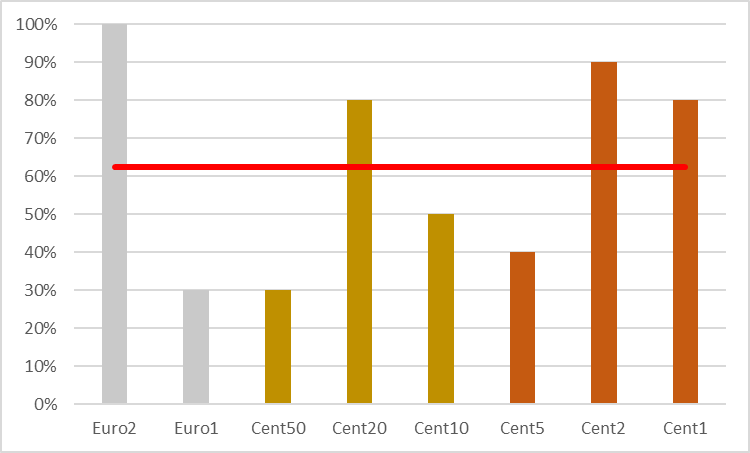
\includegraphics[width=\textwidth]{../SuccessRate2.png}  
\end{figure}

Wie man sofort sieht, gibt es starke Unterschiede in der Erfolgsrate der einzelnen Münzen. Während die 2-Euro Münze in fast allen Fällen korrekt erkannt wurde, lag die Erfolgsquote für die 1 Euro Münze nur bei etwa 30\%. Neben der 2-Euro Münze werden auch die 20-Cent, 2-Cent und 1-Cent Münzen in den meisten Fällen (>50\%) korrekt erkannt. Dagegen werden die 1-Euro, 50-Cent und 5-Cent Münzen nur in etwa 30-40\% der Fälle korrekt erkannt. Für die 10-Cent Münze liegt die Erfolgsrate bei etwa 50\%. Insgesamt beträgt die durchschnittliche Erfolgsrate für alle Münzen somit 62,5\%.

Alles in allem wieder recht durchwachsene Ergebnisse. Zwar konnte ich durch meine Änderungen die Erfolgsrate im Vergleich zu meinem letzten Blogbeitrag auf über 50\% steigern, jedoch ist dies immer noch weit von einer zuverlässigen Münzerkennung entfernt. Die Kantenerkennung scheint dabei der richtige Weg gewesen zu sein, dennoch scheint sie noch nicht einwandfrei zu funktionieren. Die Kanten-Bilder der Vorlagen sehen nahezu perfekt aus, jedoch scheinen besonders die zu prüfenden Münzen nicht immer in ein verwertbares Kantenbild umgewandelt zu werden. Es hat sich als sehr schwierig erwiesen Parameter zu finden, welche für alle Münzen ein gutes Ergebnis liefern, sodass die Konturen der Ziffer klar erkennbar sind, jedoch nicht zu viele Störungen vorhanden sind.

Ich denke jedoch, dass mich dennoch beweisen konnte, dass mittels Template-Matching und OpenCV.js eine Münzerkennung im Browser möglich ist. Die Ergebnisse könnten sicherlich mit etwas weiterem Feintuning verbessert werden, jedoch würde dies den Rahmen dieses Blogs sprengen. Jener Blog neigt sich nun auch dem Ende zu, daher möchte ich im nächsten Abschnitt noch ein Fazit ziehen und einen Ausblick auf mögliche Weiterentwicklungen geben. \newpage

\section{Fazit}

\subsection{Zusammenfassung}
Die Möglichkeit von openCV.js, OpenCV-Funktionen direkt im Browser des Clients auszuführen, eröffnet eine Vielzahl von neuen Anwendungsmöglichkeiten. Rechenintensive Bildverarbeitungsalgorithmen müssen nun nicht mehr auf einem Server laufen, wodurch Kapazitäten frei werden und für andere Aufgaben genutzt werden können. Immer mehr Onlinebesuche finden auf mobilen Geräten statt - die Verwendung der eingebauten Kamera für Bildverarbeitungsaufgaben könnte somit in Zukunft eine wichtige Rolle spielen. 

\subsection{Die größten Probleme}
Es hat sich gezeigt, dass mit openCV sehr anspruchsvolle Probleme in der Bildverarbeitung gelöst werden können. Je nach Umfang und Komplexität des Problems kann die Implementierung jedoch sehr aufwendig sein. Die größten Probleme, die ich während der Implementierung hatte, waren die folgenden:

\begin{itemize}
    \item \textbf{Dokumentation} - Speziell für OpenCV.js ist die Dokumentation sehr spärlich. Die offizielle Dokumentation ist nur für C++ verfügbar und die JavaScript-Tutorials sind oft nicht ausreichend. Zudem erschwert die Emscripten-Übersetzung den Einstieg, da in der IDE keine Autovervollständigung für die OpenCV-Funktionen verfügbar ist. Es gibt keine leichte Möglichkeit, alle Funktionen und Parameter in Erfahrung zu bringen, was die Implementierung erschwert.
    \item \textbf{Umgebungsbedingungen} - Viele Methoden der Bilderkennung haben sich als sehr empfindlich gegenüber den Umgebungsbedingungen herausgestellt. So haben beispielsweise die Lichtverhältnisse und die Kameraqualität einen großen Einfluss auf die Ergebnisse. Vor allem das Licht stellt ein nur schwer zu lösendes Problem dar, welches nur schwer "genormt" werden kann. 
    \item \textbf{Parameter} - Die Parameter der OpenCV-Funktionen sind oft sehr spezifisch und müssen genau auf den Anwendungsfall abgestimmt werden. So kann es sein, dass eine Funktion bei falscher Einstellung gar nicht oder nur sehr schlechte Ergebnisse liefert. Das Finden der richtigen Parameter hat sich als sehr zeitaufwendig herausgestellt.
\end{itemize}

\subsection{Ausblick}
Ich hoffe mit diesem Blog einen Einblick in die Möglichkeiten von OpenCV.js gegeben zu haben. Die Implementierung von Bildverarbeitungsalgorithmen im Browser ist eine spannende Entwicklung, die in Zukunft sicherlich noch an Bedeutung gewinnen wird. Selbst wenn die letztendlichen Ergebnisse des CoinFinders nicht perfekt sind, so zeigt das Projekt doch sehr gut, für welche verschiedene Anwendungsfälle OpenCV.js genutzt werden kann.

Man darf nicht vergessen, dass die Kreiserkennung und das Template-Matching, wie ich es in diesem Blog implementiert habe, nur ein kleiner Teil der Möglichkeiten von OpenCV sind. OpenCV bietet eine Vielzahl von weiteren Funktionen, die womöglich auch für das Problem des CoinFinders verwendet werden könnten. So gibt es in OpenCV weitere Möglichkeiten der Objekterkennung, welche mithilfe von Deep Neural Networks (DNN) realisiert werden. Diese sind natürlich deutlich komplizierter und aufwendiger zu implementieren als die Methoden die ich in diesem Blog vorgestellt habe, sie könnten jedoch auch deutlich bessere Ergebnisse liefern. Dies wäre eine spannende Weiterentwicklung des Projekts, welche jedoch den Scope dieses Blogs übersteigen würde.  \newpage

\end{document}